The 0D flow model offers a rapid generation of the \gls{DNP} group parameters, though it treats the flow in a simplified manner.
Rather than modeling the actual flow of the fuel salt, the residence times of the fuel salt in each region gives a rough estimate of the fuel circulation.
Figure \ref{fig:sophisticated-model} shows the flow diagram for a spatially resolved model that uses Moltres instead of OpenMC.

\begin{figure}[H]
    \centering
    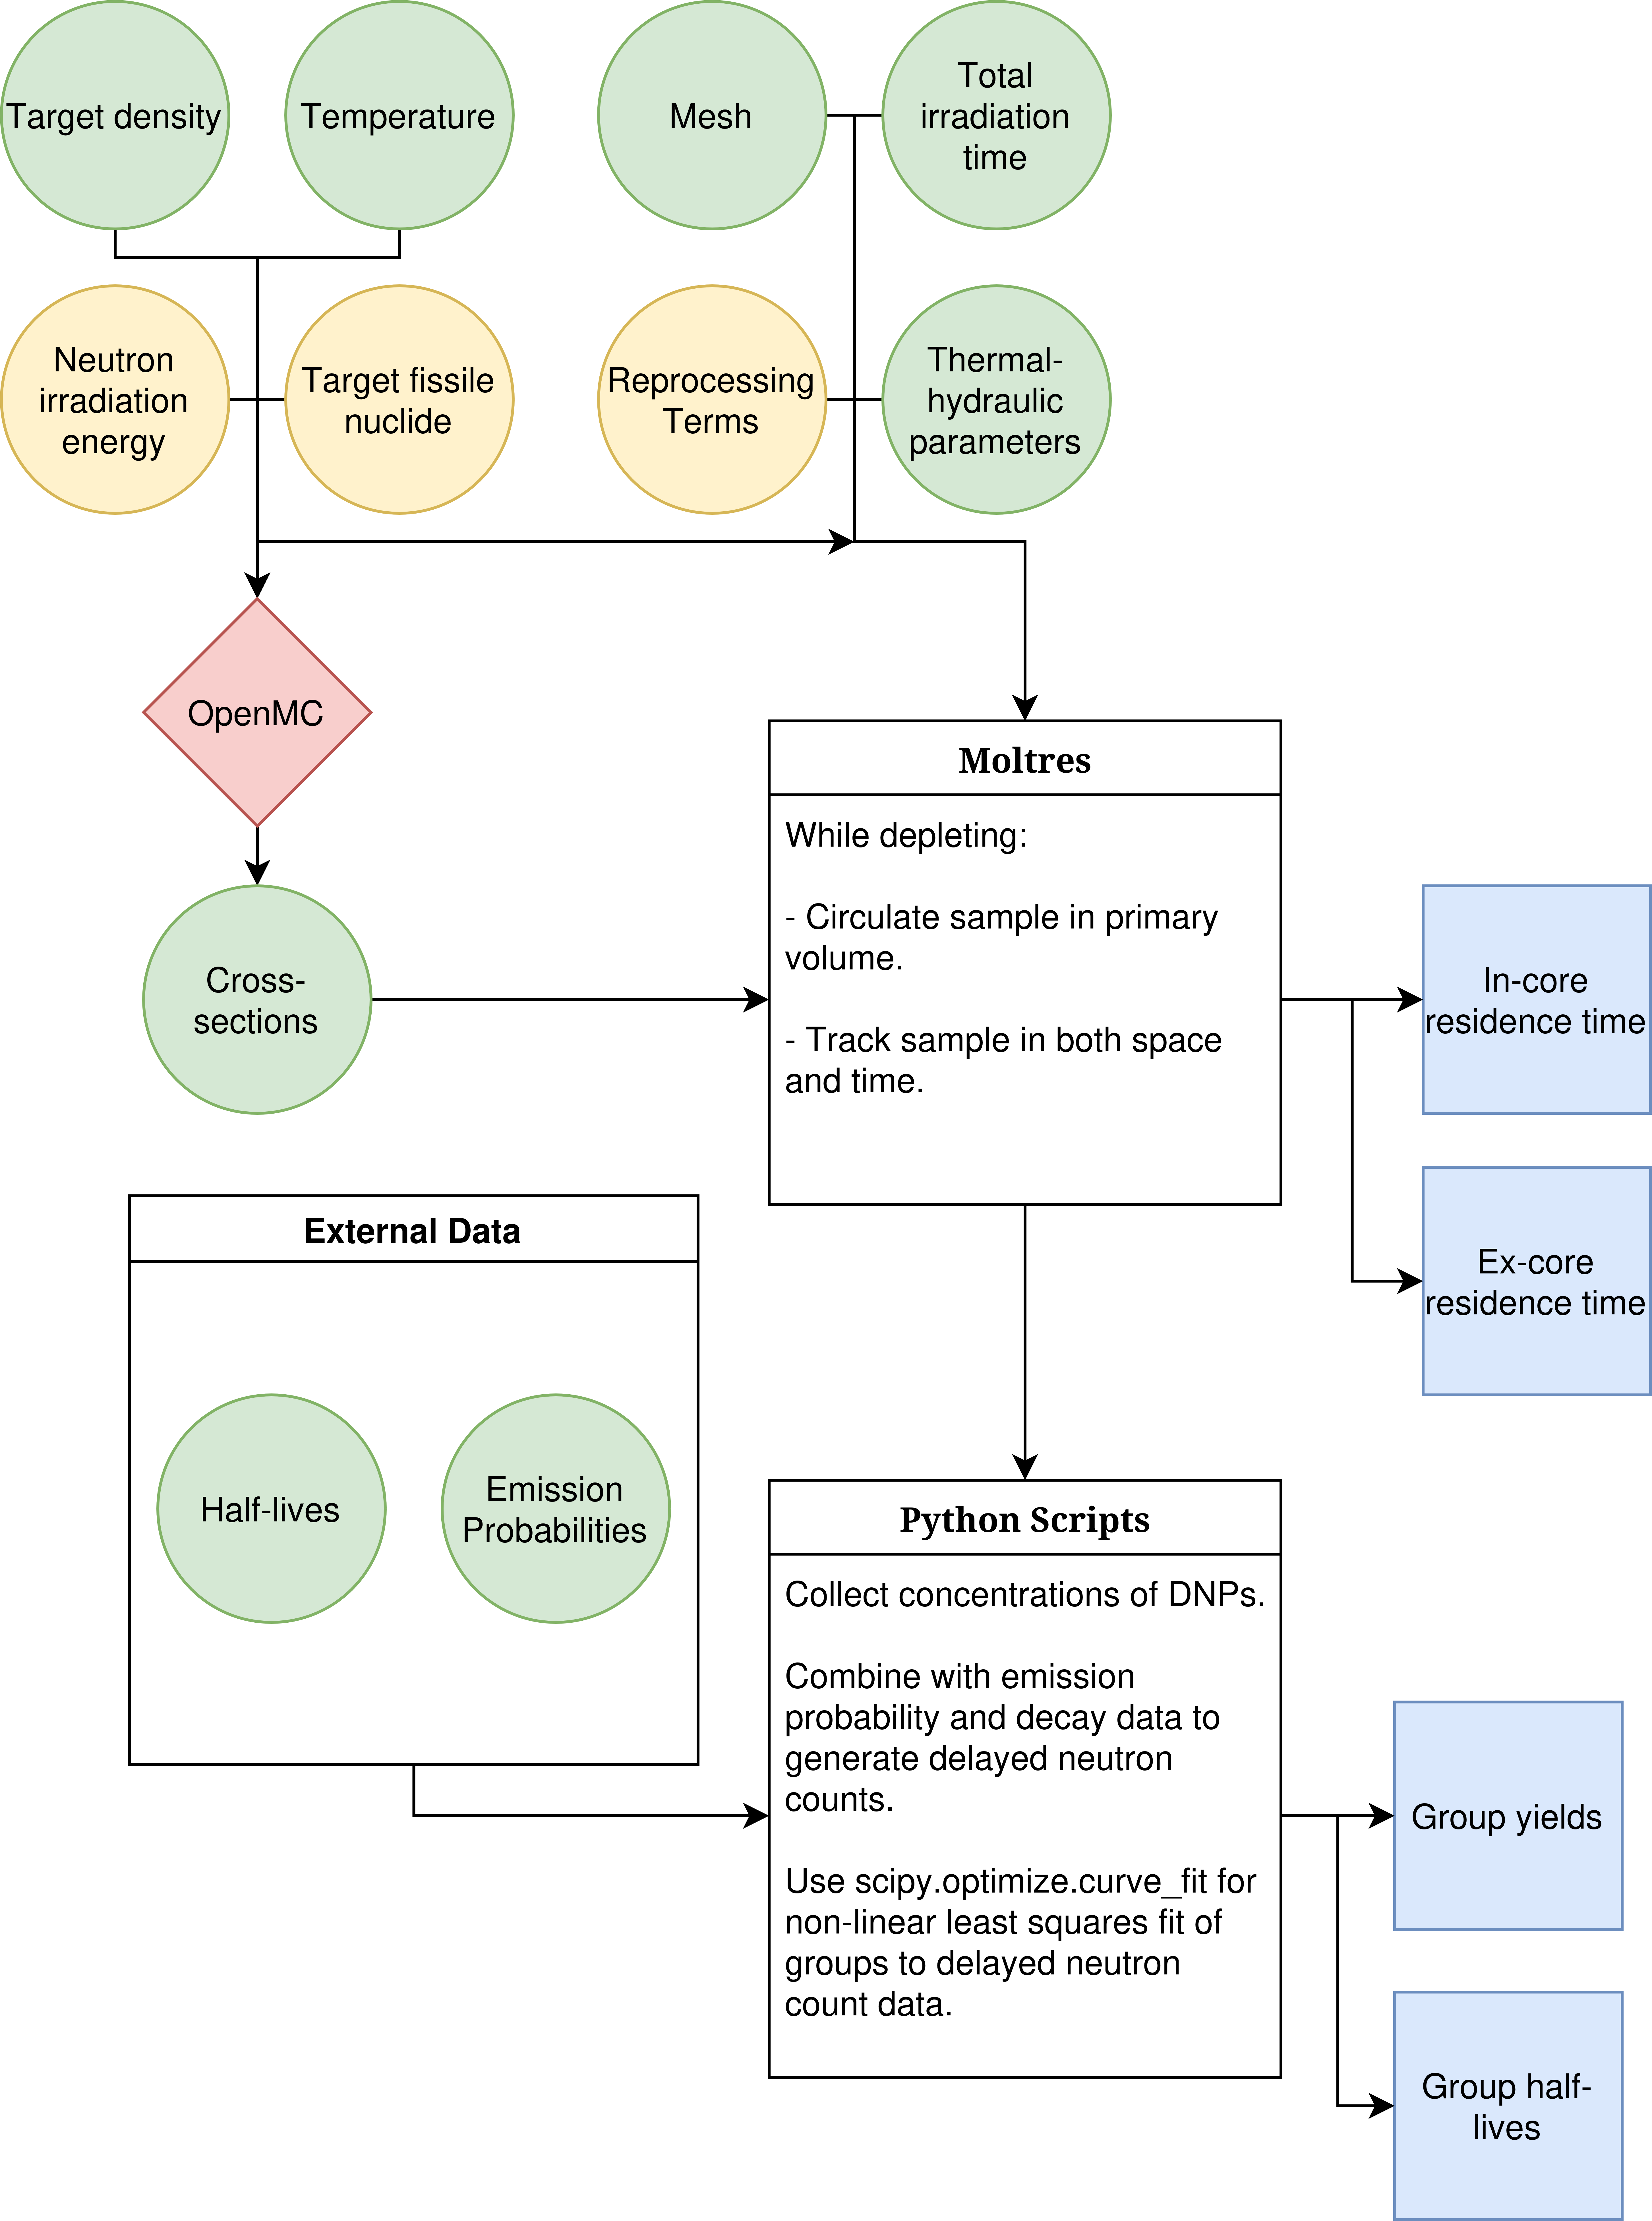
\includegraphics[width=0.9\linewidth]{images/sophisticated-model-4.png}
    \caption{Flow diagram of spatially resolved flow model used to generate flow-inclusive precursor group fit parameters.}
    \label{fig:sophisticated-model}
\end{figure}

There are two new parameters in the spatially resolved flow model that are not present in the 0D flow model.
The first is the mesh, which dictates the geometry of the problem.
MOOSE offers built-in meshing tools, though this may be insufficient depending on the complexity of the problem geometry.
In such a case, an external meshing tool, such as Gmsh, can be used \cite{geuzaine2009gmsh}.
The other new parameter is the thermal-hydraulics parameters.
This parameter captures many of the physical phenomena involved with inclusion of spatial resolution, as discussed in Section \ref{sec:moltres}.

The in-core and ex-core residence times are also outputs rather than inputs for the spatially resolved model.
This is because the residence times can be calculated from the movement of the irradiated sample over time in the fuel salt.
The in-core and ex-core residence times will change over time as the irradiated sample diffuses and mixes more in the fuel salt.
The net residence time, $\tau_{net}$, will not change over time without some change to the model such as an increased temperature difference or induced flow rate.
Equation \eqref{eq:incore-time} gives the in-core residence time as:

\begin{equation}
    \tau_{in} (t) = \frac{\int_{V_{in}} \int_{0}^t N(\vec{x}, t) dt d\vec{x}}{\int_{V} \int_{0}^t N(\vec{x}, t) dt d\vec{x}} \tau_{net},
    \label{eq:incore-time}
\end{equation}
where
\begin{align}
V_{in} &= \mbox{ the in-core volume} \nonumber \\
V &= \mbox{ the total primary volume } \nonumber \\
N(\vec{x}, t) &= \mbox{ the time and space resolved sample concentration} \nonumber \\
\tau_{net} &= \mbox{ the net residence, or circulation, time of the fuel salt.} \nonumber
\end{align}

The ex-core residence time can be calculated in the same way, or alternatively as shown in Equation \eqref{eq:excore-time} as:

\begin{equation}
    \tau_{ex} = \tau_{net} - \tau_{in}.
    \label{eq:excore-time}
\end{equation}